\documentclass[a4paper]{article}

\usepackage[T1]{fontenc}
\usepackage[utf8]{inputenc}
\usepackage{mlmodern}

%\usepackage{ngerman}	% Sprachanpassung Deutsch

\usepackage{graphicx}
\usepackage{geometry}
\geometry{a4paper, top=15mm}

\usepackage{subcaption}
\usepackage[shortlabels]{enumitem}
\usepackage{amssymb}
\usepackage{amsthm}
\usepackage{amsmath}
\usepackage{mathtools}
\usepackage{braket}
\usepackage{bbm}
\usepackage{graphicx}
\usepackage{float}
\usepackage{yhmath}
\usepackage{tikz}
\usepackage{scratch}
\usetikzlibrary{patterns,decorations.pathmorphing,positioning}
\usetikzlibrary{calc,decorations.markings}

\usepackage[backend=biber, sorting=none]{biblatex}
\addbibresource{cite.bib}

\usepackage[framemethod=TikZ]{mdframed}

\tikzstyle{titlered} =
    [draw=black, thick, fill=white,%
        text=black, rectangle,
        right, minimum height=.7cm]


\usepackage[colorlinks=true,naturalnames=true,plainpages=false,pdfpagelabels=true]{hyperref}
\usepackage[parfill]{parskip}
\usepackage{lipsum}

\usepackage{tcolorbox}
\tcbuselibrary{skins,breakable}

\pagestyle{myheadings}

\colorlet{colexam}{black}
\newcounter{definition}
\newtcolorbox[use counter=definition]{mydef}[1]{
    empty,
    title={\textbf{Definition~\thetcbcounter}~~(\textit{#1})},
    attach boxed title to top left,
    fontupper=\sl,
    boxed title style={
        empty,
        size=minimal,
        bottomrule=1pt,
        top=1pt,
        left skip=0cm,
        overlay=
            {\draw[colexam,line width=1pt]([yshift=-0.4cm]frame.north
        west)--([yshift=-0.4cm]frame.north east);}},
            coltitle=colexam,
            fonttitle=\normalfont,
            before=\par\medskip\noindent,
            parbox=false,
            boxsep=-1pt,
            left=0.75cm,
            right=3mm,
            top=4pt,
            breakable,
            pad at break*=0mm,
            vfill before first,
            overlay unbroken={
                \draw[colexam,line width=1pt]
                ([xshift=0.6cm, yshift=-0.5pt]frame.south
                west)--([xshift=0.6cm,yshift=-1pt]frame.north west)
                --([xshift=0.6cm]frame.south west)--([xshift=-13cm]frame.south east); },
            overlay first={
                \draw[colexam,line width=1pt]
                ([xshift=0.6cm, yshift=-0.5pt]frame.south
                west)--([xshift=0.6cm,yshift=-1pt]frame.north west)
                --([xshift=0.6cm]frame.south west); },
            overlay last={
                \draw[colexam,line width=1pt]
                ([xshift=0.6cm, yshift=-0.5pt]frame.south
                west)--([xshift=0.6cm,yshift=-1pt]frame.north west)
                --([xshift=0.6cm]frame.south west)--([xshift=-13cm]frame.south east); }
}
\newcounter{theorem}
\newtcolorbox[use counter=theorem]{theorem}{
    empty,
    title={Theorem ~\thetcbcounter},
    attach boxed title to top left,
    fontupper=\sl,
    boxed title style={
        empty,
        size=minimal,
        bottomrule=1pt,
        top=1pt,
        left skip=0cm,
        overlay=
            {\draw[colexam,line width=1pt]([yshift=-0.4cm]frame.north
        west)--([yshift=-0.4cm]frame.north east);}},
            coltitle=colexam,
            fonttitle=\bfseries,
            before=\par\medskip\noindent,
            parbox=false,
            boxsep=-1pt,
            left=0.75cm,
            right=3mm,
            top=4pt,
            breakable,
            pad at break*=0mm,
            vfill before first,
            overlay unbroken={
                \draw[colexam,line width=1pt]
                ([xshift=0.6cm, yshift=-0.5pt]frame.south
                west)--([xshift=0.6cm,yshift=-1pt]frame.north west)
                --([xshift=0.6cm]frame.south west)--([xshift=-13cm]frame.south east); },
            overlay first={
                \draw[colexam,line width=1pt]
                ([xshift=0.6cm, yshift=-0.5pt]frame.south
                west)--([xshift=0.6cm,yshift=-1pt]frame.north west)
                --([xshift=0.6cm]frame.south west); },
            overlay last={
                \draw[colexam,line width=1pt]
                ([xshift=0.6cm, yshift=-0.5pt]frame.south
                west)--([xshift=0.6cm,yshift=-1pt]frame.north west)
                --([xshift=0.6cm]frame.south west)--([xshift=-13cm]frame.south east); }
}
\newcounter{lemma}
\newtcolorbox[use counter=lemma]{lemma}{
    empty,
    title={Lemma~\thetcbcounter},
    attach boxed title to top left,
    fontupper=\sl,
    boxed title style={
        empty,
        size=minimal,
        bottomrule=1pt,
        top=1pt,
        left skip=0cm,
        overlay=
            {\draw[colexam,line width=1pt]([yshift=-0.4cm]frame.north
        west)--([yshift=-0.4cm]frame.north east);}},
            coltitle=colexam,
            fonttitle=\bfseries,
            before=\par\medskip\noindent,
            parbox=false,
            boxsep=-1pt,
            left=0.75cm,
            right=3mm,
            top=4pt,
            breakable,
            pad at break*=0mm,
            vfill before first,
            overlay unbroken={
                \draw[colexam,line width=1pt]
                ([xshift=0.6cm, yshift=-0.5pt]frame.south
                west)--([xshift=0.6cm,yshift=-1pt]frame.north west)
                --([xshift=0.6cm]frame.south west)--([xshift=-13cm]frame.south east); },
            overlay first={
                \draw[colexam,line width=1pt]
                ([xshift=0.6cm, yshift=-0.5pt]frame.south
                west)--([xshift=0.6cm,yshift=-1pt]frame.north west)
                --([xshift=0.6cm]frame.south west); },
            overlay last={
                \draw[colexam,line width=1pt]
                ([xshift=0.6cm, yshift=-0.5pt]frame.south
                west)--([xshift=0.6cm,yshift=-1pt]frame.north west)
                --([xshift=0.6cm]frame.south west)--([xshift=-13cm]frame.south east); }
}

\newcommand{\eps}{\varepsilon}
\usepackage[OT2,T1]{fontenc}
\DeclareSymbolFont{cyrletters}{OT2}{wncyr}{m}{n}
\DeclareMathSymbol{\Sha}{\mathalpha}{cyrletters}{"58}

\markright{Popović\hfill Seminar\hfill}


\title{University of Vienna\\
\vspace{1cm}Seminar:\\Joint RICAM Seminar\\
\vspace{0.5cm}
Summary of talk by Otmar Scherzer
}
\author{Milutin Popovic}


\begin{document}
\maketitle
\tableofcontents
\section{Introduction}
MPS or PEPS (in 2D) describe ground states of gapped local Hamiltonian of
quantum many body systems. We will use this fact to generalize Landau's
theory (to do: what is Landau's theory brief explanation, How do we describe
these with MPS in particular). Here we consider only ground states that can
be represented by MPS exactly. Two systems are in the same phase, if and only
if the can be connected by a smooth path of local Hamiltonian's on the
manifold of the parameters $\lambda$, where the local Hamiltonian's $h_i =
h_i(\lambda)$ are all dependent on the parameters $\lambda$, intuitively this
would look the figure below are all dependent on the parameters $\lambda$,
intuitively this would look the figure below.

\begin{figure}[H]
    \centering
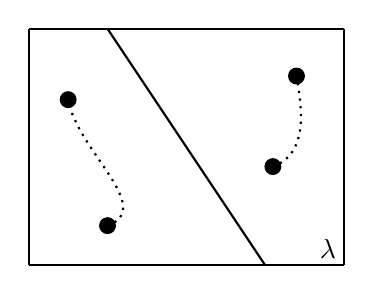
\begin{tikzpicture}[]
    \node[thick] at (3.8, 0.2) {$\lambda$};

    \draw[-, thick] (0,0)--(4,0);
    \draw[-, thick] (4,0)--(4,3);
    \draw[-, thick] (4,3)--(0,3);
    \draw[-, thick] (0,3)--(0,0);
    \draw[-, thick] (1,3)--(3,0);


    \filldraw[black] (1, 0.5) circle (0.1cm);
    \filldraw[black] (0.5, 2.1) circle (0.1cm);

%    \filldraw[black] (1.5, 1.3) circle (0.1cm);
%    \filldraw[black] (2.4, 1.8) circle (0.1cm);
%    \draw[thick, dotted] (1.5, 1.3) to[out=20, in=-80]  (2.4, 1.8);

    \filldraw[black] (3.4, 2.4) circle (0.1cm);
    \filldraw[black] (3.1, 1.25) circle (0.1cm);

    \draw[thick, dotted] (3.1, 1.25) to[out=20, in=-80]  (3.4, 2.4);
    \draw[thick, dotted] (1, 0.5) to[out=20, in=-80]  (0.5, 2.1);

\end{tikzpicture}
\caption{Two systems in the same phase are connected by a ''smooth path of local
Hamiltonians``}
\end{figure}
Where along such paths the physical properties of the sate smoothly change.
The Hamiltonian needs to be ''gapped``, meaning that there is a clear
separation of the ground state and the first excited state. The loss of a
gap in the Hamiltonian leads mostly to discontinuous ``behavior'' of the ground
state and affection of global properties of the system. If we introduce
symmetries along the path of such Hamiltonian we can derive a refined
classification of phases. Additionally if such symmetries exist we  can
generalize gapped quantum phases to systems with symmetry breaching!
%\printbibliography
\section{Matrix Product States (MPS)}
In the following we only consider translation-invariant systems on a finite
chain of length $N$, with periodic boundary condition
\begin{mydef}
    Consider a spin chain $(\mathbb{C}^{d})^{\otimes N}$. A
    translation-invariant MPS $\ket{\mu[\mathcal{P}]}$ of bond dimension $D$
    on $(\mathbb{C}^{d})^{\otimes N}$ is constructed by placing maximally
    entangled pairs $\ket{\omega_D}$, as
    \begin{align}
        \ket{\omega_D} := \sum_{n=1}^{D} \ket{i, i}
    \end{align}
    between adjacent sites and applying a linear map $\mathcal{P}:
    \mathbb{C}^{D} \otimes  \mathbb{C}^{D} \rightarrow \mathbb{C}^{d}$. In
    graphical notation it would represent the figure below
    \begin{figure}[H]
        \centering
    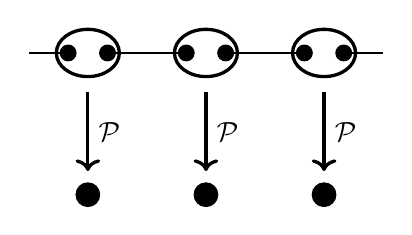
\begin{tikzpicture}[]
        \filldraw[black] (0, 0) circle (0.1cm);
        \filldraw[black] (0.5, 0) circle (0.1cm);

        \filldraw[black] (1.5, 0) circle (0.1cm);
        \filldraw[black] (2, 0) circle (0.1cm);

        \filldraw[black] (3, 0) circle (0.1cm);
        \filldraw[black] (3.5, 0) circle (0.1cm);

        \draw[-, thick] (-0.5, 0) -- (0, 0);
        \draw[-, thick] (0.5, 0) -- (1.5, 0);
        \draw[-, thick] (2, 0) -- (3, 0);
        \draw[-, thick] (3.5, 0) -- (4, 0);

        \draw[very thick] (0.25,0) ellipse (0.4cm and 0.3cm);
        \draw[very thick] (1.75,0) ellipse (0.4cm and 0.3cm);
        \draw[very thick] (3.25,0) ellipse (0.4cm and 0.3cm);

        \draw[->, very thick] (0.25, -0.5) -- (0.25, -1.5) node[midway, right] {$\mathcal{P}$};
        \draw[->, very thick] (1.75, -0.5) -- (1.75, -1.5) node[midway, right] {$\mathcal{P}$};
        \draw[->, very thick] (3.25, -0.5) -- (3.25, -1.5) node[midway, right] {$\mathcal{P}$};

        \filldraw[black] (0.25, -1.8) circle (0.15cm);
        \filldraw[black] (1.75, -1.8) circle (0.15cm);
        \filldraw[black] (3.25, -1.8) circle (0.15cm);

    \end{tikzpicture}
    \end{figure}
    \begin{align}
        \ket{\mu[\mathcal{P}]} := \mathcal{P}^{\otimes N}\ket{\omega_D}^{\otimes N}
    \end{align}
\end{mydef}
We note that the MPS as defined above is robust under blocking sites, we are
essentially blocking $k$-sites into one ''super``-site of dimension $d^k$,
which gives a new MPS with the same bond dimension in the lines of the
projector (which is not a projection but a simple linear map)
\begin{align}
    \mathcal{P}' = \mathcal{P}^{\otimes k} \ket{\omega_D}^{\otimes (k-1)}.
\end{align}
By this blocking and using of the gauge degrees of freedom (including the
variability of $D$) any MPS which is well defined in the Thermodynamic limit
($\beta \rightarrow 0$) can be brought into a so called \textbf{Standard
form}, where the linear map $\mathcal{P}$ is supported on a block-diagonal
space, i.e diagonalisation of the
\begin{align}
    \text{ker}(\mathcal{P})^{\perp} =
    \mathcal{H}_1 \oplus \cdots \oplus \mathcal{H}_{\mathcal{A}},
\end{align}
where
\begin{align}
    \mathcal{H}_\alpha = \text{span}\left\{ \ket{i, j}: \zeta_{\alpha- 1}<
    i,j \le \zeta_\alpha \right\},
\end{align}
for $0 = \zeta_0 < \cdots < \zeta_\mathcal{A} = D$, and gives the
partitioning $1, \ldots, D$ for $D_i = \zeta_i - \zeta_{i-1}$. The case of
$\mathcal{A}=1$ we have an injective map $\mathcal{P}$. The $\mathcal{A} >1$
is the non-injective case.

All in all we assume that $\mathcal{P}$ is \textbf{surjective}, which is
backed by the restriction of the state space $\mathbb{C}^{d}$ to the image of
$\mathcal{P}$ (by definition).
\subsection{Parent Hamiltonian}
Given an MPS in the standard form, we can construct local,
translation-invariant \textbf{parent Hamiltonians}, which have the given MPS
as the \textbf{ground state}
\begin{align}\label{eq: hamiltonian}
   H = \sum_{i=1}^{N} h(i,i+1).
\end{align}
The local terms $h(i, i+1) \ge 0$ act on one MPS object $(i, i+1)$ mapped by
$\mathcal{P}$. The kernels of these local terms support the reduced density
operator of the corresponding MPS, that is the kernel can be written as
\begin{align}
    \text{ker}(h(i,i+1)) = (\mathcal{P} \otimes
    \mathcal{P})(\mathbb{C}^{D}\otimes \ket{\omega} \otimes \mathbb{C}^{D}).
\end{align}
Note that by the definition we have first that $H \ge 0$, and that
$H\ket{\mu[\mathcal{P}]} = 0$, because the system $\ket{\mu[\mathcal{P}]}$ is
the ground state of $H$.
\newline

To summarize, given a matrix product state (MPS) there exists a unique gapped
local parent Hamiltonian, where the given MPS is in the groundstate
(Perez-Garcia et al. 2007). Also, backed up by the fact that the groundstate
of any one dimensional, gapped Hamiltonian can be well approximated by an MPS
(proven by Hastings 2007).
\subsection{Definition of quantum phases}
We arrive at the definition of quantum phases, where we initially pose a
question whether two systems are in the same phase. Two systems are in the
same phase if they can be connected by a continuous path of gapped local
Hamiltonians
\subsubsection{Phases without symmetries}
Let $H_1, H_2$ be a family of translation-invariant gapped local Hamiltonians
on a ring (i.e. periodic boundary conditions). We say that $H_1$ and $H_2$
are in the same phase, if and only if exists an finite $k$, when blocking $k$
sites both $H_1$ and $H_2$ are two local and can be written as
\begin{align}
    H_p = \sum_{i=1}^{N} h_p(i,i+1) \qquad p=0,1.
\end{align}
Additionally to this there exists a translation-invariant path of local
gapped Hamiltonians
\begin{align}
    H_\gamma = \sum_{i=1}^{N} h_\gamma(i,i+1) \qquad \gamma \in [0, 1],
\end{align}
where $h_\gamma$ is acting locally with the following properties
\begin{itemize}
    \item $h_0 = h_{\gamma=0}$ ; $h_1 = h_{\gamma=1}$
    \item $\|h\|_{op} \le 1$
    \item $h_\gamma$ is continuous w.r.t. $\gamma \in [0, 1]$
    \item $H_\gamma$ has a spectral gap above the ground state manifold,
        bounded below by  some constant $\Delta >0$ independent of $N$ and
        $\gamma$.
\end{itemize}
We can say that $H_0$ and $H_1$ are in the same phase if they are connected
by a local, bound-strength, continuous and gapped path, which applies to both
Hamiltonians with unique and degenerate ground states.
\subsubsection{Phases with symmetries}
Let $H_p$, with $p \in \left\{ 0, 1 \right\} $ be a Hamiltonian acting on the
space $\mathcal{H}^{\otimes N}_p$ where $\mathcal{H}_p=\mathbb{C}^{d_p}$ and
$U_g^p$ be a linear unitary representation of some group $G \ni g$ of
$\mathcal{H}_p$. Now, $U_g$ is a symmetry of a family of local gapped
Hamiltonians $H_p$, if
\begin{align}
    [H_p, (U_g^p)^{\otimes N}] = 0 \qquad \forall g\in G,
\end{align}
where $U_g^p$ is a strictly one dimensional representation of the group $G$
as
\begin{align}
    U_g^p \leftrightarrow e^{i\phi_g^p}U_g^p.
\end{align}
We can say that $H_1$ and $H_2$ are in the same phase under symmetry $G$, if
there exists a phase gauge of $U_g^0$ and $U_g^1$ and a representation
\begin{align}
     U = U_g^0 \oplus U_g^1 \oplus U_g^{\alpha} \qquad \alpha \in (0, 1)
\end{align}
on the Hilbertspace $\mathcal{H} = \mathcal{H}_0 \oplus  \mathcal{H}_1 \oplus
\mathcal{H}_\alpha$ with the properties of the previous section, such that
\begin{align}
    [H_\gamma, U_g^{\otimes N}] = 0
\end{align}
and $H_p$ is supported on $\mathcal{H}_p$ for $p=0, 1$ respectively.
\subsubsection{Robust definition of Phases}
It is usually required for a phase to be \textbf{robust}, meaning that the
phase is an open set in the space of allowed Hamiltonians. For all
Hamiltonians \ref{eq: hamiltonian} there exists and $\varepsilon >0$, such
that
\begin{align}
    H = \sum_{i=1}^{N} \left( h(i,i+1) + \varepsilon k(i, i+1) \right)
\end{align}
is in the same phase for any bound-strength $k(i,i+1)$ which obeys the
symmetries of the system.
\subsubsection{Restriction to parent Hamiltonians}
Indeed we want a classification of phases of gapped local Hamiltonians with an
exact MPS ground state. We are in luck because for every MPS we can find such
a Hamiltonian, the parent Hamiltonian which is sufficient enough to classify
the phases.

For two gapped Hamiltonians $H, H'$ with some ground state subspace, the
interpolating path
\begin{align}
    \gamma H + (1-\gamma)H'
\end{align}
has all the desired properties and it is gapped. Indeed all parent
Hamiltonians for a given MPS are interchangeable!

\begin{figure}[H]
    \centering
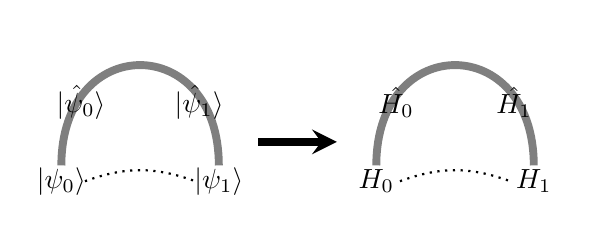
\begin{tikzpicture}[]
    \node[thick] at (0, 0) {$\ket{\psi_0}$};
    \node[thick] at (2, 0) {$\ket{\psi_1}$};
    \node[thick] at (0.25, 1) {$\ket{\hat{\psi}_0}$};
    \node[thick] at (1.75, 1) {$\ket{\hat{\psi}_1}$};

    \node[thick] at (4, 0) {$H_0$};
    \node[thick] at (6, 0) {$H_1$};
    \node[thick] at (4.25, 1) {$\hat{H_0}$};
    \node[thick] at (5.75, 1) {$\hat{H_1}$};

    \draw[thick, dotted] (0.3, 0) to[out=20, in=160]  (1.7, 0);
    \draw[thick, dotted] (4.3, 0) to[out=20, in=160]  (5.7, 0);

    \draw[line width=0.1cm, opacity=0.5] (0, 0.2) to[out=90, in=90,
        distance=1.7cm]  (2, 0.2);
    \draw[line width=0.1cm, opacity=0.5] (4, 0.2) to[out=90, in=90,
        distance=1.7cm]  (6, 0.2);

    \draw[-stealth, line width=0.1cm] (2.5, 0.5) -- (3.5, 0.5);



\end{tikzpicture}
\caption{Interchangeability of MPS and parent Hamiltonians}
\end{figure}
\subsection{The isometric Form}
\subsubsection{Reduction to a standard form}
Given two MPS $\ket{\mu [\mathcal{P}_p]}$ with $p=0,1$ together with their
nearest neighbor parent Hamiltonians $H_p$. Our goal is to see weather $H_1$
and $H_2$ are in the same phase. This is achieved by interpolating
$\mathcal{P}_0$ and $\mathcal{P}_1$ along $\mathcal{P}_\gamma$, such that the
result is the path $H_\gamma$ in the space of parent Hamiltonians satisfying
all the requirements (continuity and gap).
\subsubsection{The isometric form}
The isometric form of a MPS captures the essential entanglement, long
range properties of the sate and forms a fixed point of a renormalization
procedure. Given an MPS state $\ket{\mu[\mathcal{P}]}$ we decompose
$\mathcal{P}$ by the \textbf{Polar-decomposition} of
$\mathcal{P}|_{(\text{ker}\mathcal{P})^\perp}$ as
\begin{align}
    \mathcal{P} = QW,
\end{align}
where $WW^\dagger= \mathbbm{1}$ and $Q > 0$. And w.l.o.g. we assume $0<Q\le
\mathbbm{1}$ which can be achieved by rescaling of $\mathcal{P}$. The
isometry form of $\ket{\mu[\mathcal{P}]}$ is $\ket{\mu[W]}$, where the MPS
described by $W$ is the isometric part of the tensor $\mathcal{P}$. To see
that $\ket{\mu[\mathcal{P}]}$ and $\ket{\mu[W]}$ are in the same phase, we
essentially define an interpolating path in terns of $Q_\gamma$
\begin{align}
    \mathcal{P}_\gamma = Q_\gamma W \quad \text{where} \quad
    Q_\gamma = \gamma Q + (1-\gamma)\mathbbm{1},
\end{align}
for $\gamma \in [0, 1]$. No consider the parent Hamiltonian of
$\ket{\mu[\mathcal{P}_0]}$
\begin{align}
    H_0 = \sum_{i=1}^{N}h_0 (i, i+1)
\end{align}
where $h_0$ is a projector and we define $\Lambda_\gamma =
(Q^{-1}_\gamma)^{\otimes  2}$ for a $\gamma$-deformed Hamiltonian
\begin{align}
    H_\gamma = \sum_{i=1}^{N} h_\gamma(i, i+1) \quad \text{where} \quad
    h_\gamma =
    \Lambda_\gamma h_0 \Lambda_\gamma \ge 0.
\end{align}
Now we have that $\ket{\mu[\mathcal{P}_0]} = 0$ is equivalent to
$\ket{\mu[\mathcal{P}_\gamma]} = 0$, i.e. $H_\gamma$ is a parent Hamiltonian
of $\ket{\mu[\mathcal{P}_\gamma]}$. All we need to show now is that
$H_\gamma$ is uniformly gapped, that there exists a constant $\Delta >0$
which $H_\gamma$ by bellow independent of $\gamma$ and $N$. By this we would
have that the whole set of $\ket{\mu[\mathcal{P}_\gamma]}$ for $\gamma \in
[0, 1]$ are indeed in the same phase.

Additional observation is that the lower bound of the gapped parent
Hamiltonians is bound by correlation length $\xi$ of the gap $H_\gamma$,
restricted to $\xi$ sites and since both depend smoothly, positive definite
on $\gamma$ and $\xi \rightarrow 0$ as $\gamma \rightarrow 0$ we have a
uniform lower bound on the gap.
\end{document}

